\newaufgabe{
Implementieren sie (natürlich unter zu-Hilfenahme einer AES realisierenden Library)
ECM und CBC unter AES selbst und bestätigen sie experimentell das beschriebene
Verhalten von CBC bei Ciphertextfehlern. Vergleichen sie weiters ihre ECM und
CBC Varianten mit den Varianten die die Library zur Verfügung stellt bzgl. der
benötigten Rechenzeit.
}
Der Code für die Block-Cipher-Modi wurde in Rust geschrieben und getestet. 
Für diesen Zweck wurde eine \texttt{encrypt} und eine \texttt{decrypt} erstellt,
die als Parameter den zu verwendenden Modus erhalten. 
\begin{minted}{rust}
pub fn encrypt<T: AsRef<[u8]>>(
        msg: T, 
        key: &[u8; 16], 
        mode: BlockCipherMode
    ) -> Vec<u8> {
    // ...
    match mode {
        BlockCipherMode::ECM => 
            ecm::encrypt(msg, Aes128::new(key)),
        BlockCipherMode::CBC(iv) => 
            cbc::encrypt(msg, Aes128::new(key), iv)
        _ => msg,
    }
}
\end{minted}
Die \texttt{decrypt} Methode funktioniert analog. Die ECM Methoden
teilen zuerst die Nachricht in 16 Byte (128 Bit) große Blöcke auf und verschlüsseln
jeden einzeln.
\begin{minted}{rust}
// ECM MODE
pub fn encrypt(mut msg: Vec<u8>, cipher: Aes128) -> Vec<u8> {
    msg.chunks_exact_mut(16)
        .map(GenericArray::from_mut_slice)
        .for_each(|block| cipher.encrypt_block(block));
    msg
}

pub fn decrypt(mut msg: Vec<u8>, cipher: Aes128) -> Vec<u8> {
    msg.chunks_exact_mut(16)
        .map(GenericArray::from_mut_slice)
        .for_each(|block| cipher.decrypt_block(block));
    msg
}
\end{minted}
Beim CBC Modus wird zusätzlich der voherige Ciphertextblock gespeichert und vor der
verschlüsselung mit dem aktuellen Block geXORed. Im Fall des ersten Blocks, ist der
vorherige der Initialisierungsvektor (IV).
\begin{minted}{rust}
// CBC MODE
pub fn encrypt(mut msg: Vec<u8>, cipher: Aes128, iv: [u8; 16]) -> Vec<u8> {
    let mut prev = &GenericArray::from(iv);
    for block in msg
        .chunks_exact_mut(16)
        .map(GenericArray::<u8, U16>::from_mut_slice)
    {
        block.iter_mut().zip(prev).for_each(|(a, &b)| *a ^= b);
        cipher.encrypt_block(block);
        prev = block;
    }
    msg
}
\end{minted}
Die Entschlüsselung im CBC Modus erfolgt in umgekehrter Reihenfolge. Durch einen
\texttt{Peekable}-Iterator kann während der Iteration über die Blöcke einfach über
\texttt{peek()} auf den darauffolgenden Block zugegriffen werden. 
Gibt es kein darauffolgendes Element, wir stattdessen der 
Initialisierungsvektor verwendet.
\begin{minted}{rust}
pub fn decrypt(mut msg: Vec<u8>, cipher: Aes128, iv: [u8; 16]) -> Vec<u8> {
    let mut block_iter = msg
        .chunks_exact_mut(16)
        .map(GenericArray::<u8, U16>::from_mut_slice)
        .rev()
        .peekable();

    while let Some(block) = block_iter.next() {
        let prev = match block_iter.peek() {
            Some(b) => b,
            None => &GenericArray::from(iv),
        };

        cipher.decrypt_block(block);
        block.iter_mut().zip(prev).for_each(|(a, &b)| *a ^= b);
    }

    msg
}
\end{minted} 

\paragraph{Verhalten bei Bitfehlern} Ausgehend von einem quadratischen, einfarbigen Bild wird
jeweils die Verschlüsselung und die Entschlüsselung mit ECM oder CBC durchgeführt.
\begin{table}
    \begin{center}
        \begin{tabular}{|c|c|c|c|}
        \hline
        Modus &Plain & Verschlüsselt & Entschlüsselt\\
        \hline
        ECM &
        
\includegraphics[width=3cm]{img/no_error/original} &
        
\includegraphics[width=3cm]{img/no_error/output_ECM} &
        
\includegraphics[width=3cm]{img/no_error/output_ECM_decrypt} \\
        \hline
        CBC &
        
\includegraphics[width=3cm]{img/no_error/original} &
        
\includegraphics[width=3cm]{img/no_error/output_CBC} &
        
\includegraphics[width=3cm]{img/no_error/output_CBC_decrypt} \\
        \hline
        \end{tabular}   
    \end{center}
    \caption{Verschlüsselung \& Entschlüsselung ohne Bitfehler}
\end{table}
\begin{table}
    \begin{center}
        \begin{tabular}{|c|c|c|c|}
        \hline
        Modus &Plain & Verschlüsselt & Entschlüsselt\\
        \hline
        ECM &
        
\includegraphics[width=3cm]{img/error/original} &
        
\includegraphics[width=3cm]{img/error/output_ECM} &
        
\includegraphics[width=3cm]{img/error/output_ECM_decrypt} \\
        \hline
        CBC &
        
\includegraphics[width=3cm]{img/error/original} &
        
\includegraphics[width=3cm]{img/error/output_CBC} &
        
\includegraphics[width=3cm]{img/error/output_CBC_decrypt} \\
        \hline
        \end{tabular}   
    \end{center}
    \caption{Verschlüsselung \& Entschlüsselung mit Bitfehler}
    \label{tab:biterror}
\end{table}
In Tabelle \ref{tab:biterror} ist zu erkennen, dass die Fehlerfortpflanzung den Erwartungen entspricht.
\newpage
\paragraph{Benchmarking}
\begin{figure}[h]
    \centering
    \begin{subfigure}[b]{0.49\textwidth}
        \centering
        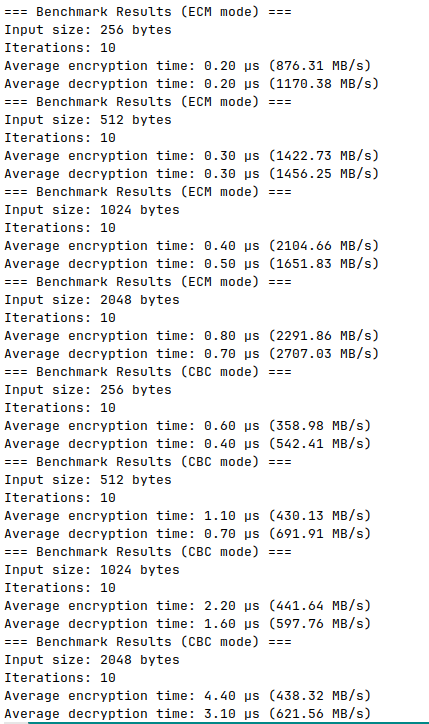
\includegraphics[width=\textwidth]{img/bench/custombench}
        \caption{Meine Implementation}
        \label{fig:bench_my}
    \end{subfigure}
    \hfill
    \begin{subfigure}[b]{0.49\textwidth}
        \centering
        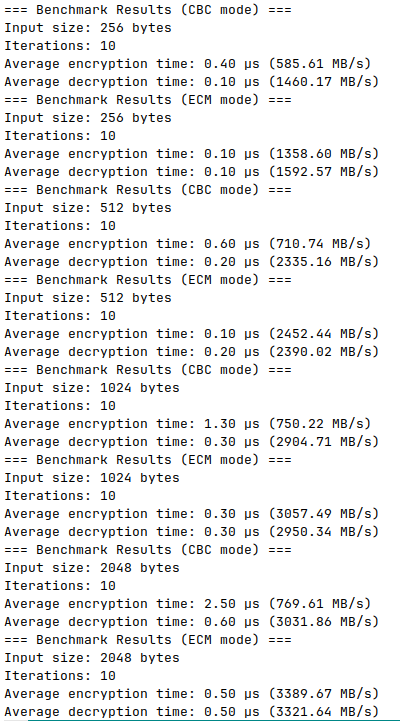
\includegraphics[width=\textwidth]{img/bench/referencebench.png}
        \caption{Referenz Implementation}
        \label{fig:bench_ref}
    \end{subfigure}
    \caption{Geschwindigkeitsvergleich}
    \label{fig:benchmark}
\end{figure}
Die Werte zeigen, dass meine eigene Implementation stellenweiße so schnell wie
die Referenz Implementation ist. Bei größeren Plaintexten wird meine Implementation langsamer,
wogegen die Referenz konstanter (und sogar teilweise schneller) ist. 